\section{Formal Models of the Environment}
\label{formalModelsofEnv}
To perform closed-loop model checking of medical devices, we need formal models of their physiological environment to represent different physiological conditions the devices may encounter. In this section, implantable pacemakers are used as example. Timed-automata \cite{timed_automata} models of the human heart are developed as the environment model \cite{sttt13,VHM_proc}. Physiological requirements are formalized with monitors and TCTL formula  \cite{TCTL}. Model checking can then be performed on the closed-loop system in model checker UPPAAL \cite{uppaal}. %The physiological knowledge required during closed-loop model checking of medical devices are associated with the \emph{physiological models} and the \emph{physiological requirements}. It is thus important to maintain the physiological context of the models and link model behaviors to physiological requirements. In this section we use heart modeling as example to demonstrate physiological knowledge encoding. %First, we introduce the physiological basis for our heart modeling. Then we demonstrate our heart model structure which can be used to model different heart conditions. We link transitions in the models to physiological behaviors
\begin{figure}[!t]
	\centering
	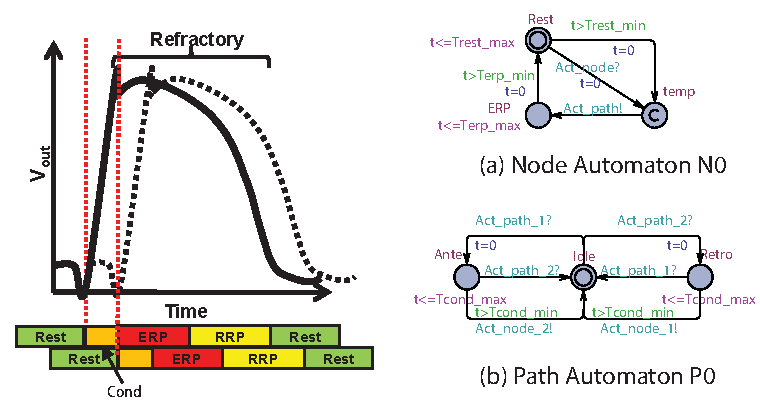
\includegraphics[width=0.9\textwidth]{figs/init_abs.pdf}
	%\vspace{-5pt}
	\caption{\small (a) Action potential for a heart tissue and its tissue nearby (dashed). (b) Node automaton. (c) Path automaton. (d) An example model of the heart consist of a network of node and path automata}
	\label{fig:nodepathTA}
\end{figure}

\subsection{Timed-automata Models of the Heart}
At cellular level, a heart tissue can be activated by external voltage. Certain tissue also has capability to self-activate, which contribute to natural heart beats. Once activated (Marker 1 in \figref{nodepathTA}), the voltage outside the tissue changes over time, which is referred to as \emph{Action Potential} (\figref{nodepathTA}.(a)). The action potential can be divided into two functional timing periods: The \emph{Effective Refractory Period (ERP)}, during which the tissue cannot be triggered by another activation; and the \emph{Rest} period, during which the tissue can be activated and at the end of which the tissue will self-activate. The timing behaviors of the action potential are modeled as \emph{node automaton} (\figref{nodepathTA}.(b)). A node automaton initializes with \textsf{Rest} state.
From \textsf{Rest} state, the node can either self-activate or be activated by external activations (indicated by Act\_node). Upon activation the node transition to the \textsf{ERP} state and activate all the paths connecting to the node (indicated by Act\_path). 
In the \textsf{ERP} state the node does not respond to external activations. At the end of \textsf{ERP} state the node transition to the \textsf{Rest} state. The time a node automaton can stay in each state is from a non-deterministic range $[Trest\_min,Trest\_max]$.
For heart tissue without the capability to self-activate, the parameters $Trest\_min$ and $Trest\_max$ are set to $\infty$.

The voltage change of the heart tissue will activate the tissue nearby with certain delay (Marker 2 in \figref{nodepathTA}). This timing delay between heart tissue is modeled using \emph{path automata} (\figref{nodepathTA}.(c)). The initial state of a path automaton is \textsf{Idle}, which corresponds to no conduction. 
A path has two conduction directions, forward and backward.
These are represented by the states \textsf{Ante} and \textsf{Retro}, named after their standard physiological terms Antegrade and Retrograde.
If \textsf{Act\_path} event is received from one of the nodes (1 or 2) connected to the path, the a transition to \textsf{Ante} or \textsf{Retro} state will occur in the path automaton. 
At the end of \textsf{Ante} and \textsf{Retro} state the path will transition to \textsf{Idle} state and send Act\_node signal to the node automaton connected to the other end of the path (2 or 1).

A healthy heart generates periodic electrical impulses to control heart rates according to physiological needs. These impulses propergate through the heart, triggering coordinated muscle contractions and pump blood to the rest of the body. The underlying pattern and timing of these impulses determine the heart's rhythm and are the key to proper heart functions. Derangements in this rhythm are referred to as \emph{arrhythmia}, which impair the heart's ability to pump blood and compromise the patients' health. Arrhythmia are categorized into so-called \textsf{Tachycardia} and \textsf{Bradycardia}. Tachycardia features undesirable fast heart rate which results in inefficient blood pumping. Bradycardia features slow heart rate which results in insufficient blood supply. Different heart conditions can be distinguished by the \emph{timing} of the electrical conduction, and the \emph{topology} of the electrical conduction system of the heart, which are researched in clinical setting referred to as \emph{Electrophysiology (EP)}\cite{josephson}. Heart tissue can be modeled as \emph{Node automata} and the conduction delays between nodes are modeled as \emph{Path automata} (\figref{nodepathTA}). 


%\subsection{Timed-automata Models of the Heart}
%\label{labeledGraph}
%In a healthy heart, specialized tissue in the \emph{SA node} self-activate periodically. The signal conducts throughout both atria, causing them to contract and push the blood into the ventricles
%Models of different physiological conditions have to be developed to be able to interact with the medical devices. This initial set of physiological models should be able to distinguish the physiological conditions that each model represents. Ideally the models are developed using formalisms that are suitable for provable abstraction and model checking. 

%A node automaton models the conduction states of heart tissue, and changes therein. 
%Its three states correspond to 3 timing periods of the action potential. 
%From \textsf{Rest} state, the node can either self-activate or be activated by external stimuli (both events are indicated by Act\_node) and transition to the \textsf{ERP} state. 
%In the \textsf{ERP} state the node does not respond to external stimuli because it is refractory. 
%In the \textsf{RRP} state, the node can still be activated and transition to the \textsf{ERP} state.
%But the fact that the activation arrived early (in the RR Period) affects the ERP and the conduction delay of the tissue.  
%%This is tracked by a shared variable $C(i)$ for the $i^{th}$ node automaton. \todo[inline]{what is $C$?}
%%The new ERP period is determined by a function over clock value $g(f(t))$ which mimics the beat-to-beat dynamics described in \cite{josephson}. \todo[inline]{what are $g,f$?}
%
%The electrical conduction through the tissue \emph{between} nodes is abstracted using \emph{path automata}. 
%The path automata are used to represent structural or functional electrical connections between nodes. 
 
%%At the same time the clock invariant of the state is modified according to the shared variable $C(a/b)$. 
%%This corresponds to the change of the conduction delay that is caused by early activation. 
%Similarly to a node automaton, the changing trend is extracted from clinical data. 
%
%The parameters of the node and path automata determine the ranges of time in which the automata can stay in corresponding locations. 
%The lower endpoint is specified as a clock invariant and the upper endpoint is specified as a guard. 
%For a heart model $G$ with $n$ nodes and $m$ paths (thus, $n$ vertices and $m$ edges), the node automata are denoted as $N_i, i\in[n]$ and path automata are denoted as $P_j,j\in[m]$. 
%\todo[inline]{change to $V_i$ and $E_i$ to stay consistent with definition of graph?}
%The parameters for the nodes are $Trest$ (with range $[Trest_{min}$),TERP,TRRP and the parameters for the paths are $\{Tante,Tretro\}$. 
The spatial and temporal properties of a given human heart condition can be modeled by a network of node and path automata with different parameters (i.e. \figref{nodepathTA}.(d)). Physiological structures of the heart are represented as node automata and the path automata specifies the connectivities of the nodes and the conduction delays among them. The network can be viewed as a labeled directed graph: %the vertices of the graph represent nodes, or locations, in the heart, while edges represent conduction paths between the nodes. 
\begin{defn}
	\label{def:labeledGraph}
	[Labeled graph]
	A \textbf{labeled graph} is a directed graph $G = (V,E,A)$ where 
	$V$ is a finite set of vertices, $E \subset V\times V$ is a finite set of directed edges,
	and $A$ is a total labeling function $A: V \cup E \rightarrow TA$
	where $TA$ is the set of parametrized timed automata.
	The function $A$ labels each vertex with a \emph{node automaton}, and each edge with an \emph{path automaton}.
	All node (resp. path) automata share the same structure, and differ only in the values of their parameters.
	%The parameters of a timed automaton are variables that appear in the right-hand side of guard and invariant conditions, and whose value can only be changed by a reset that occurs at a transition.	
	%Both node and path automata are shown in Fig.~\ref{fig:nodepathTA}
\end{defn}
The heart model structure has been used to model various heart conditions and all of them have been validated by Electrophysiologists \cite{vhm_ecrts10,vhm_embc10}.

The implantable cardiac pacemakers are rhythm management devices designed to treat bradycardia. A typical dual chamber pacemaker has two leads inserted into the heart through the veins which can measure the local electrical activities of the right atrium and right ventricle, respectively. According to the timing between sensed impulses the pacemaker can deliver electrical pacing to the corresponding chamber to maintain proper heart rhythm (\figref{probes}).  
\begin{figure}[!t]
	\centering
	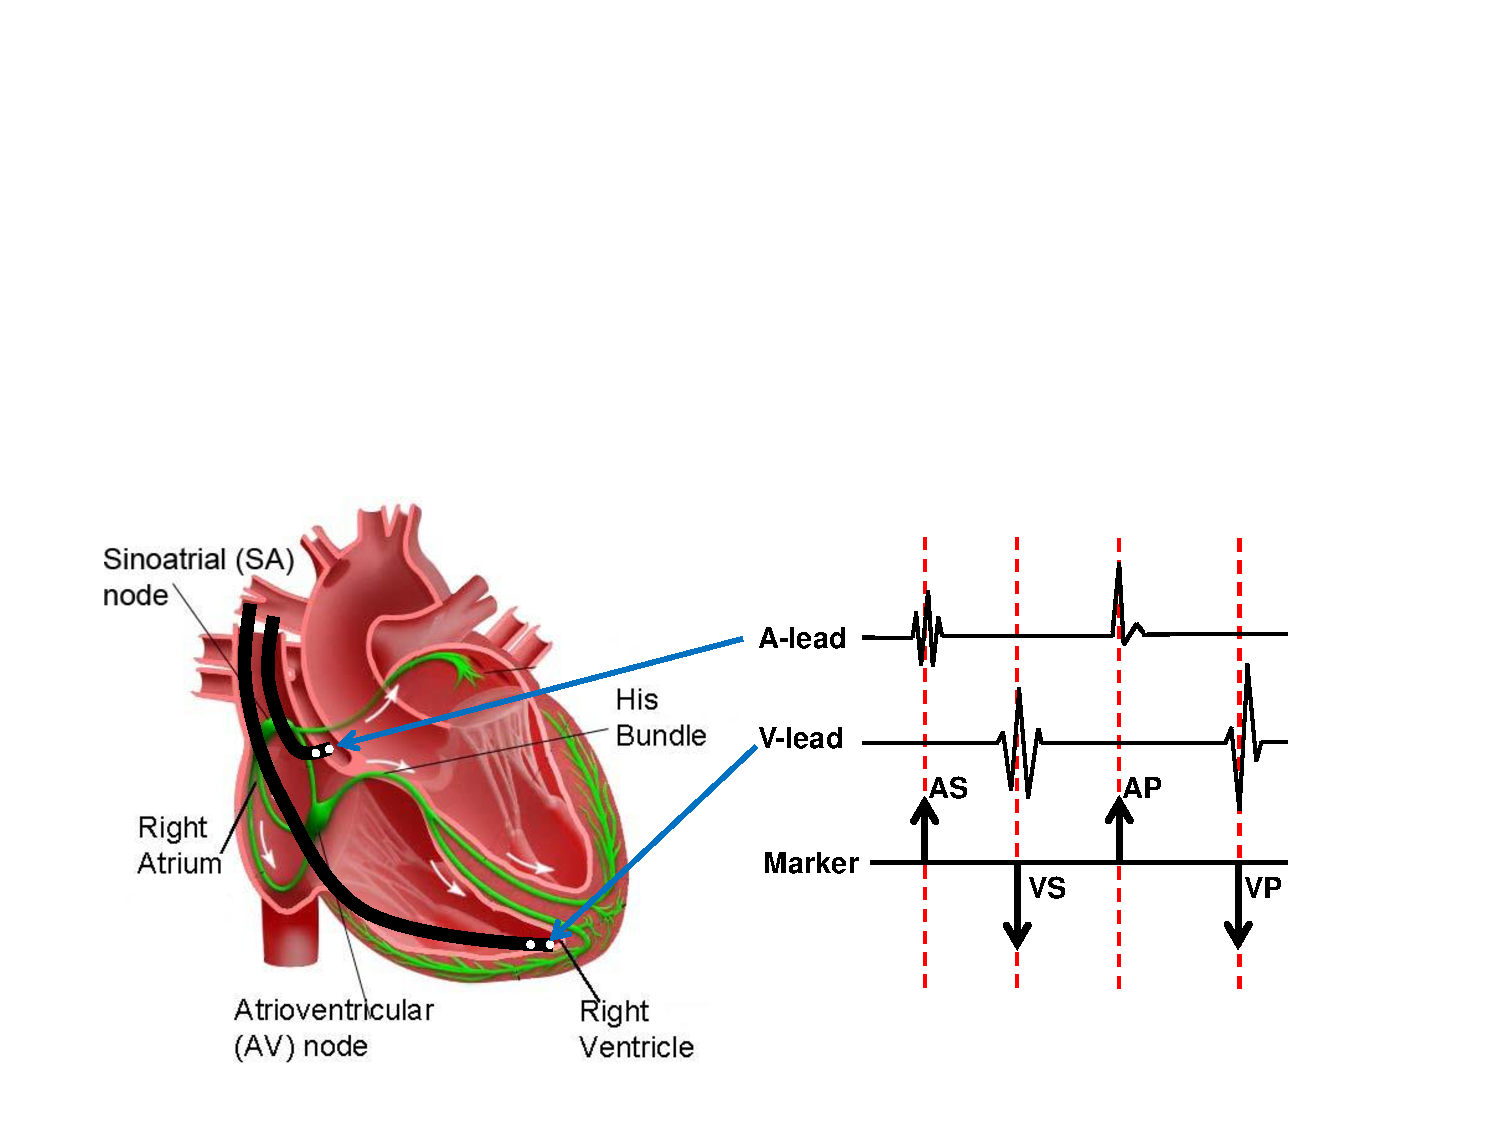
\includegraphics[width=0.7\textwidth]{figs/egm.pdf}
	
	%\vspace{-10pt}
	\caption{\small (a) Lead placement for a dual chamber pacemaker (b) Electrogram (EGM) signals from pacemaker leads and corresponding internal event markers}
	\label{fig:probes}
	%\vspace{-15pt}
\end{figure} 


%\subsection{Describe Model Behaviors with Physiological Context}
%During model abstractions, the abstract model covers all transitions of the more refined model. Transitions corresponding to physiological behaviors may be merged or replaced by other transitions. Without documenting these information, the abstract models lose their physiological context. 
%In the heart models we modeled physiological timing periods using locations in timed automata. The minimum time an automaton can stay in those locations is limited by the guard on a transition out of the location, and the maximum time is limited by the clock invariant of the state. 
%The transitions of heart tissue can be categorized into 3 basic transition groups:
%\begin{itemize}
%	\item \textbf{self:} The self-activation of the node automata. The \emph{min} and \emph{max} parameters equal to $Trest\_min$ and $Trest\_max$ parameters in the node automata, which specify the minimum and maximum intervals between consecutive self-activation events.
%
%	\item \textbf{block:} The blocking property of the node automata. The \emph{min} and \emph{max} parameters equal to $Terp\_min$ and $Terp\_max$ parameters in the node automata, which specify the minimum and maximum intervals between consecutive activations that can trigger path conduction.	
%	\item \textbf{cond:} The conduction property of the path automata. The \emph{min} and \emph{max} parameters equal to $Tcond\_min$ and $Tcond\_max$ parameters in the node automata, which specify the minimum and maximum delays between a node activation on one end and the activation on the other end.
%\end{itemize}
%As an example, a node automata $NA$ has two transition groups, which can be represented by $NA.self$ and $NA.block$

\subsection{Formalizing Physiological Requirements}
%Devices are designed to improve certain physiological conditions, the performance of the devices is evaluated on the difference between the patient conditions without the device and with the device. The device should also avoid deteriorating certain patient conditions, physiological requirements are specified in the form of:
%$$C_{pre}\rightarrow C_{post}$$
%in which $C_{pre}$ is the physiological conditions without the device,  and $C_{post}$ is the physiological condition with the device. For model-based closed-loop verification, $C_{pre}$ is often in form of a set of constraints on patient parameters. As a special case, $C_{pre}$ can equal to $true$, means that $C_{post}$ should be satisfied under all possible conditions.
%
%Physiological requirements are constraints on physiological behaviors. In \cite{iccps10} we 
%
%\subsection{Monitors}
Physiological requirements must be formalized for closed-loop model checking. In the case of medical devices, the devices are designed to \emph{improve} certain physiological conditions. 
%For an unhealthy open-loop physiological condition that a device is designed to improve, the closed-loop condition should be healthy.
Software developers are particularly interested in the scenario in which a healthy open-loop physiological condition became an unhealthy closed-loop condition due to device intervention, which is a bug in the device.

In general, a closed-loop requirement $\varphi$ is in the form of $\varphi_E\Rightarrow \varphi_C$, in which $\varphi_E$ is the open-loop physiological condition that the device encounters, often in form of parameter ranges in the environment models, and $\varphi_C$ is the closed-loop physiological condition that the device should achieve. Then we have:
\begin{equation}\label{req_def}
M_E\models\varphi_E, M_E||M_D\models \varphi_C\Rightarrow M_E||M_D\models\varphi
\end{equation}
%A requirement $\varphi: \varphi_E\Rightarrow \varphi_C$ contains open-loop environmental constraints in $\varphi_E$ and desired closed-loop condition specified in $\varphi_C$.  
The substates for a heart model are clocks and locations for each node and path automata. In \cite{vhm_iccps11}, physiological heart conditions are mapped to constraints on substate variables of the heart models, which can be written as atomic propositions. General monitors are also developed in Stateflow \cite{stateflow} for closed-loop testing of physiological requirements. The timed-automata version are shown in \figref{monitor}. The $M_{sing}(event,thresh\_min, thresh\_max)$ enforces the time interval between two $event$ signals within $[thresh\_min,thresh\_max]$. \\
$M_{doub}(event1,event2,thresh\_min,thresh\_max)$ enforces the time interval between $event1$ and $event2$ signals within $[thresh\_min,thresh\_max]$. Model checking is performed on the closed-loop system including the heart model $M_H$, the pacemaker model $M_P$, and the monitor $M$. The requirement $\varphi_P$ can be then represented with TCTL formula:
 \textsf{A[] (not M.Err)}
\begin{figure}[!b]
		\centering
		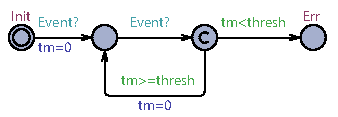
\includegraphics[width=0.8\textwidth]{figs/monitor.pdf}
		%\vspace{-5pt}
		\caption{\small (a) $M_{sing}$ for single event; (b) $M_{doub}$ for two events}
		  %\vspace{-15pt}
		\label{fig:monitor}
\end{figure}
%\section{State Space Formulation}
\label{[statespaceformulation]}
Kripke structure $<S,\Sigma,L,I>$ in which $S$ is a set of states, $\sigma(s_1,s_2)\in\Sigma\subset S^2$ is a set of transitions, $I\subset S$ is a non-empty set of initial states.

To clarify things, we first introduce \emph{state groups} and \emph{transition groups}. The state space is defined by state variables. 
$$s\{\theta_1,\theta_2\dots \theta_n\}\in S$$
Each state $s$ is a valuation of all the state variables. Partial valuations can be used to represent a state group. For example, $s\{\theta_1=v_1\}$ represents all states in which $\theta_1=v_1$.

Each state transition $\sigma\in\Sigma$ is defined as $\sigma(s_1,s_2)$ such that:
$$s_1\xrightarrow{\sigma}s_2\text{ in which }s_1,s_2\in S$$
Certain transitions have the same behaviors, mostly observablly equivalent . It is convinient to group them together to describe the behaviors of the system. A \textsf{transition group} is a group of transitions that the pre- and post- states satisfy certain criteria:
$$\Sigma_\phi\subset\Sigma \text{ s.t. }\forall\sigma(s_1,s_2)\in\Sigma_\phi,f(s_1,s_2)\models\phi,s_1,s_2\in S$$
in which $f(s_1,s_2)$ is certain proposition of the two states or their substates. It is possible that $\Sigma_{\phi_1}\cap\Sigma_{\phi_2}\neq \emptyset$.

Ideal execution path of length n: $\delta:s_0\sigma_0\dots\sigma_i\dots\sigma_ns_n\in\Sigma^*$ in which: 
$$s_0\in I, \sigma_i(s_i,s_{i+1})\in\Sigma, i\in[0,n-1]$$ 
The set of all the transitions in a path is represented by $\Sigma_\delta$.

Each transition takes time. We denote it as $t=T(\sigma)$. The time for each execution path: $$T(\delta)=\sum_{i=0}^nT(\sigma_i)$$

Partial paths: Not all the transitions in a path are necessary. In fact, ideal paths are not possible, so do ideal models. One way to represent partial paths is timed execution path: sequence of transitions with unobservable ones abstracted with time lapse $\delta_t\in(\sigma_o,t)^*, t\in \mathbb{R}$

$\delta_t$ is an abstraction of $\delta$, we denote it as $\delta\models\delta_t$. For a execution path 
$$\delta=\sigma_0\sigma_1\dots\sigma_n$$
there is a corresponding timed execution path 
$$\delta^t=(\sigma_0^t,t_0)(\sigma_1^t,t_1)\dots(\sigma_m^t,t_m)$$ 
in which
$$\forall i,j,k \text{ s.t. } \sigma_i=\sigma_k^t,\sigma_j=\sigma_{k+1}^t,(\sigma_{i+1}\dots\sigma_{j-1})\neq\sigma_{j},T(\sigma_i\dots\sigma_j)=t_{k+1}-t_k$$
with length $m<n$ such that $\delta\triangleleft\delta^t$. 

Execution path produceable by model
$$\delta\in^p M$$
\subsection{A1: Observability Distinction}
The lowest distinction requirement for a model

The most basic observable transitions are input and output of the entity under modeling

Input triggered transitions $\Sigma_i$

Output inducing transitions $\Sigma_o$

If we have a timed trace such that $\delta\triangleleft\delta_t$, all the transitions in a path $\delta$ which are input/output transitions should be preserved in the timed trace $\delta_t$. 
%$$\delta\triangleleft\delta^t\rightarrow\forall \sigma\in(\Sigma_i\cup\Sigma_o)\cap\Sigma_\delta,\sigma\in\Sigma_(\delta_t)$$

A model $M$ is observability distinctive iff
$$\forall\delta^t\in^p M, \forall\delta\triangleleft\delta^t,\forall \sigma\in(\Sigma_i\cup\Sigma_o)\cap\Sigma_\delta,\sigma\in\Sigma_{\delta^t}$$
The observability of the system and the environment are different. After the system has been developed, the observability of the environment is fixed. However, for the system itself, the observability can range from full white-box (code level) to full blackbox (input-output only)

\subsection{A2: Property Distinction}
We refer a model $M$ is property distinctive for property $\phi$ by $M\triangle\phi$, such that

$$\forall \delta^t\in^p M, \delta^t\models\phi\leftrightarrow\forall \delta\triangleleft\delta^t,  \delta\models\phi$$
%$$\forall \delta_1,\delta_2\triangleleft\delta_t, \delta_1\models\phi\leftrightarrow \delta_2\models\phi$$

\subsection{A3: Validity Distinction}


For system model $M^s$
$$\delta^t\in^p M^s \text{ iff }\exists\delta\triangleleft\delta^t\text{ s.t. } \delta\in^p M^s$$


There can be multiple execution path correspond to the same timed execution path. 
$$\exists \delta_1,\delta_2\text{ s.t. } \delta_1\models\delta_t,\delta_2\models\delta_t$$
In this case, we say that $\delta_1$ and $\delta_2$ are not \textbf{distinguishiable}. 

Distinguishible transitions: a lot of the times two paths have to be distinguishible (healthy vs. unhealthy)


Trace produceable by model: For an execution path $\delta$ with length $n$, we denote that the path is produceable by model $M$ with $\delta\triangleleft M$, such that:
$$\forall \sigma(s_i,s_{i+1})\in \delta,i\in[0,n-1], s_0\in I, \sigma(s_i,s_{i+1})\in\Sigma_M$$

Timed trace produceable by model:


non-determinism

For system:
$$\delta\models\delta_t,\delta_t\triangleleft M_s \text {  iff  } \delta\triangleleft M_s$$
For environment:
$$\delta$$
%\section{Model Abstraction With Over-approximation}
%For two models $M_1$ and $M_2$, we denote $M_2$ is an abstraction of $M_1$ as $M_1\preceq M_2$. A function $s'=h(s),s\in S_1,s'\in S_2$ is a mapping from the states in $M_1$ to states in $M_2$. 
%
%For two models $M_1$ and $M_2$ such that $M_1\preceq M_2$, we know that all the transitions are preserved:
%$$\forall \sigma(s,s') \in\Sigma_1\text{ s.t. }s,s'\in S_1,\rightarrow\sigma(h(s),h(s')) \in\Sigma_2,h(s),h(s')\in S_2$$
%Due to the mapping the transition groups in $M_2$ are changed as well. For a transition group in $M_1$:
%$$\Sigma_{\phi1}\subset\Sigma_1 \text{ s.t. }\forall\sigma(s_1,s_2)\in\Sigma_{\phi1},f(s_1,s_2)\models\phi1,s_1,s_2\in E_1$$
%In the more abstract model, the propsition is often relaxed. For certain $\phi2\supseteq\phi1$, we have:
%$$\Sigma_{\phi2}\subset\Sigma_2 \text{ s.t. }\forall\sigma(h(s_1),h(s_2))\in\Sigma_{\phi2},f(h(s_1),h(s_2))\models\phi2,s_1,s_2\in S_1$$
%
%
%Some of the transition groups are merged. For two transition groups $\Sigma_{\phi1},\Sigma_{\phi2}\subset\Sigma_1$ there exists a new relation $\Sigma_{\phi3}\subseteq\Sigma_2$ such that: $$\phi1\cup\phi2\subseteq\phi3$$
%We denote this abstraction as:
%$$\Sigma_{\phi3}=\{\Sigma_{\phi1},\Sigma_{\phi2}\}$$
%We use $\Sigma_{\phi1}\lhd\Sigma_{\phi3}$ to represent the abstraction relationship between transition groups.
%\begin{itemize}
	%\item Over-approximation and its information loss
    %\item Abstraction in terms of transition groups
    %
%\begin{itemize}
	%\item Merging
    %\item \textcolor{red}{Remove}
%\end{itemize}
	%\item Assumptions made to simplify the model and increase model behaviors
    %\item Necessity of model refinements due to information loss
%\end{itemize}
%
%\subsection{System model vs. Environment model}
%\begin{itemize}
	%\item System model achieves simplicity during abstraction
    %\item Environment model also use abstraction to achieve generalization
    %\item Validation of counter-example cannot be done on a generalized environment model
%\end{itemize}

\section{\textcolor{red}{Requirement Encoding}}
\begin{itemize}
	\item Differentiate requirements from specifications.
    \item Requirements are environmental behaviors that the system want to achieve.
    \item It countains a pre-condition and post-condition, which can be linked to transition groups.
    \item 
\end{itemize}
